\section{Online evaluation}
\begin{itemize}
	\item In online evaluation, the system interacts with the user $\implies$ user "tells" what is relevant, system analyzes the user's behavior for gaining that knowledge
	\item The benefit of online evaluations is that they are mostly simpler and directly incorporate measuring the ranking quality
	\item However, the downsides are that the results are worse to explain/interpret (why did users click less, different queries might rely on different metrics, ...). Also, evaluations might not be comparable over time so that we also need to ensure the same conditions/user population for both systems.
\end{itemize}
\subsection{Analyzing user behavior}
\begin{itemize}
	\item A user provides various signals from which we can try to retrieve his "happiness" about the results. The following ones are mostly used:
	\item \textit{Clicks} - clicks are mostly noisy so that a click doesn't ensure that the document was actually relevant. Clicks have several biases:
	\begin{itemize}
		\item \textit{Position bias} - a user tends towards clicking higher ranked results
		\item \textit{Contextual bias} - nearby results effect the click probability of a document
		\item \textit{Attention bias} - some results draw more attention to themselves by the usage of images, font size, ...
	\end{itemize}
	\item \textbf{Time} - the time a user spends on a certain query before coming back to search engine
	\begin{itemize}
		\item \textit{Dwell time} - time spent on a clicked page. If duration is more than 30 seconds, we assume that click satisfied
		\item \textit{Exit type} - how the user exists the page (closing browser, continue scrolling through results, putting in new query, ...) 
	\end{itemize}
	\item \textit{Mouse movement} - time on website is not sufficient. Mouse movement can indicate whether user is actually reading or only scrolling/scanning
	\item \textit{Reformulations} - if new query is entered, check for similarity with the previous one. Reformulated/Similar queries that were entered quickly after the first one, indicate that user was not satisfied with previous results.
\end{itemize}
\subsection{A/B Testing}
\begin{itemize}
	\item When testing two systems in an online experiment, we need to make sure that both have the same preconditions so that the system improvements clearly correlate with the new click/sale numbers
	\item In A/B Testing, users are split into two groups where each group is assigned to one of the algorithms. We analyze the users' behavior on both systems and calculate a metric based on that. Comparing the results for both systems on significance leads to a final decision.
	\item \textit{Challenges} in A/B Testing
	\begin{itemize}
		\item If one system is very different and probably bad, it will affect the \textit{user experience} and damages website image $\implies$ perform offline evaluation in advance to avoid testing a very bad system
		\item It is hard to define \textit{metrics} as they can contradict each other. For example, if we report number of clicks and sessions per users, a click increase can indicate better/more relevant results. However, if another systems provides snippets that already contain the information, the user will click less.
		\item The metric should be as sensitive as possible. \textit{Sensitivity} is the ability of the metric to detect the statistically significant difference when the treatment effect exists $\implies$ how many queries/days/users/... for significance needed?
	\end{itemize}

	\begin{figure}[ht]
		\centering
		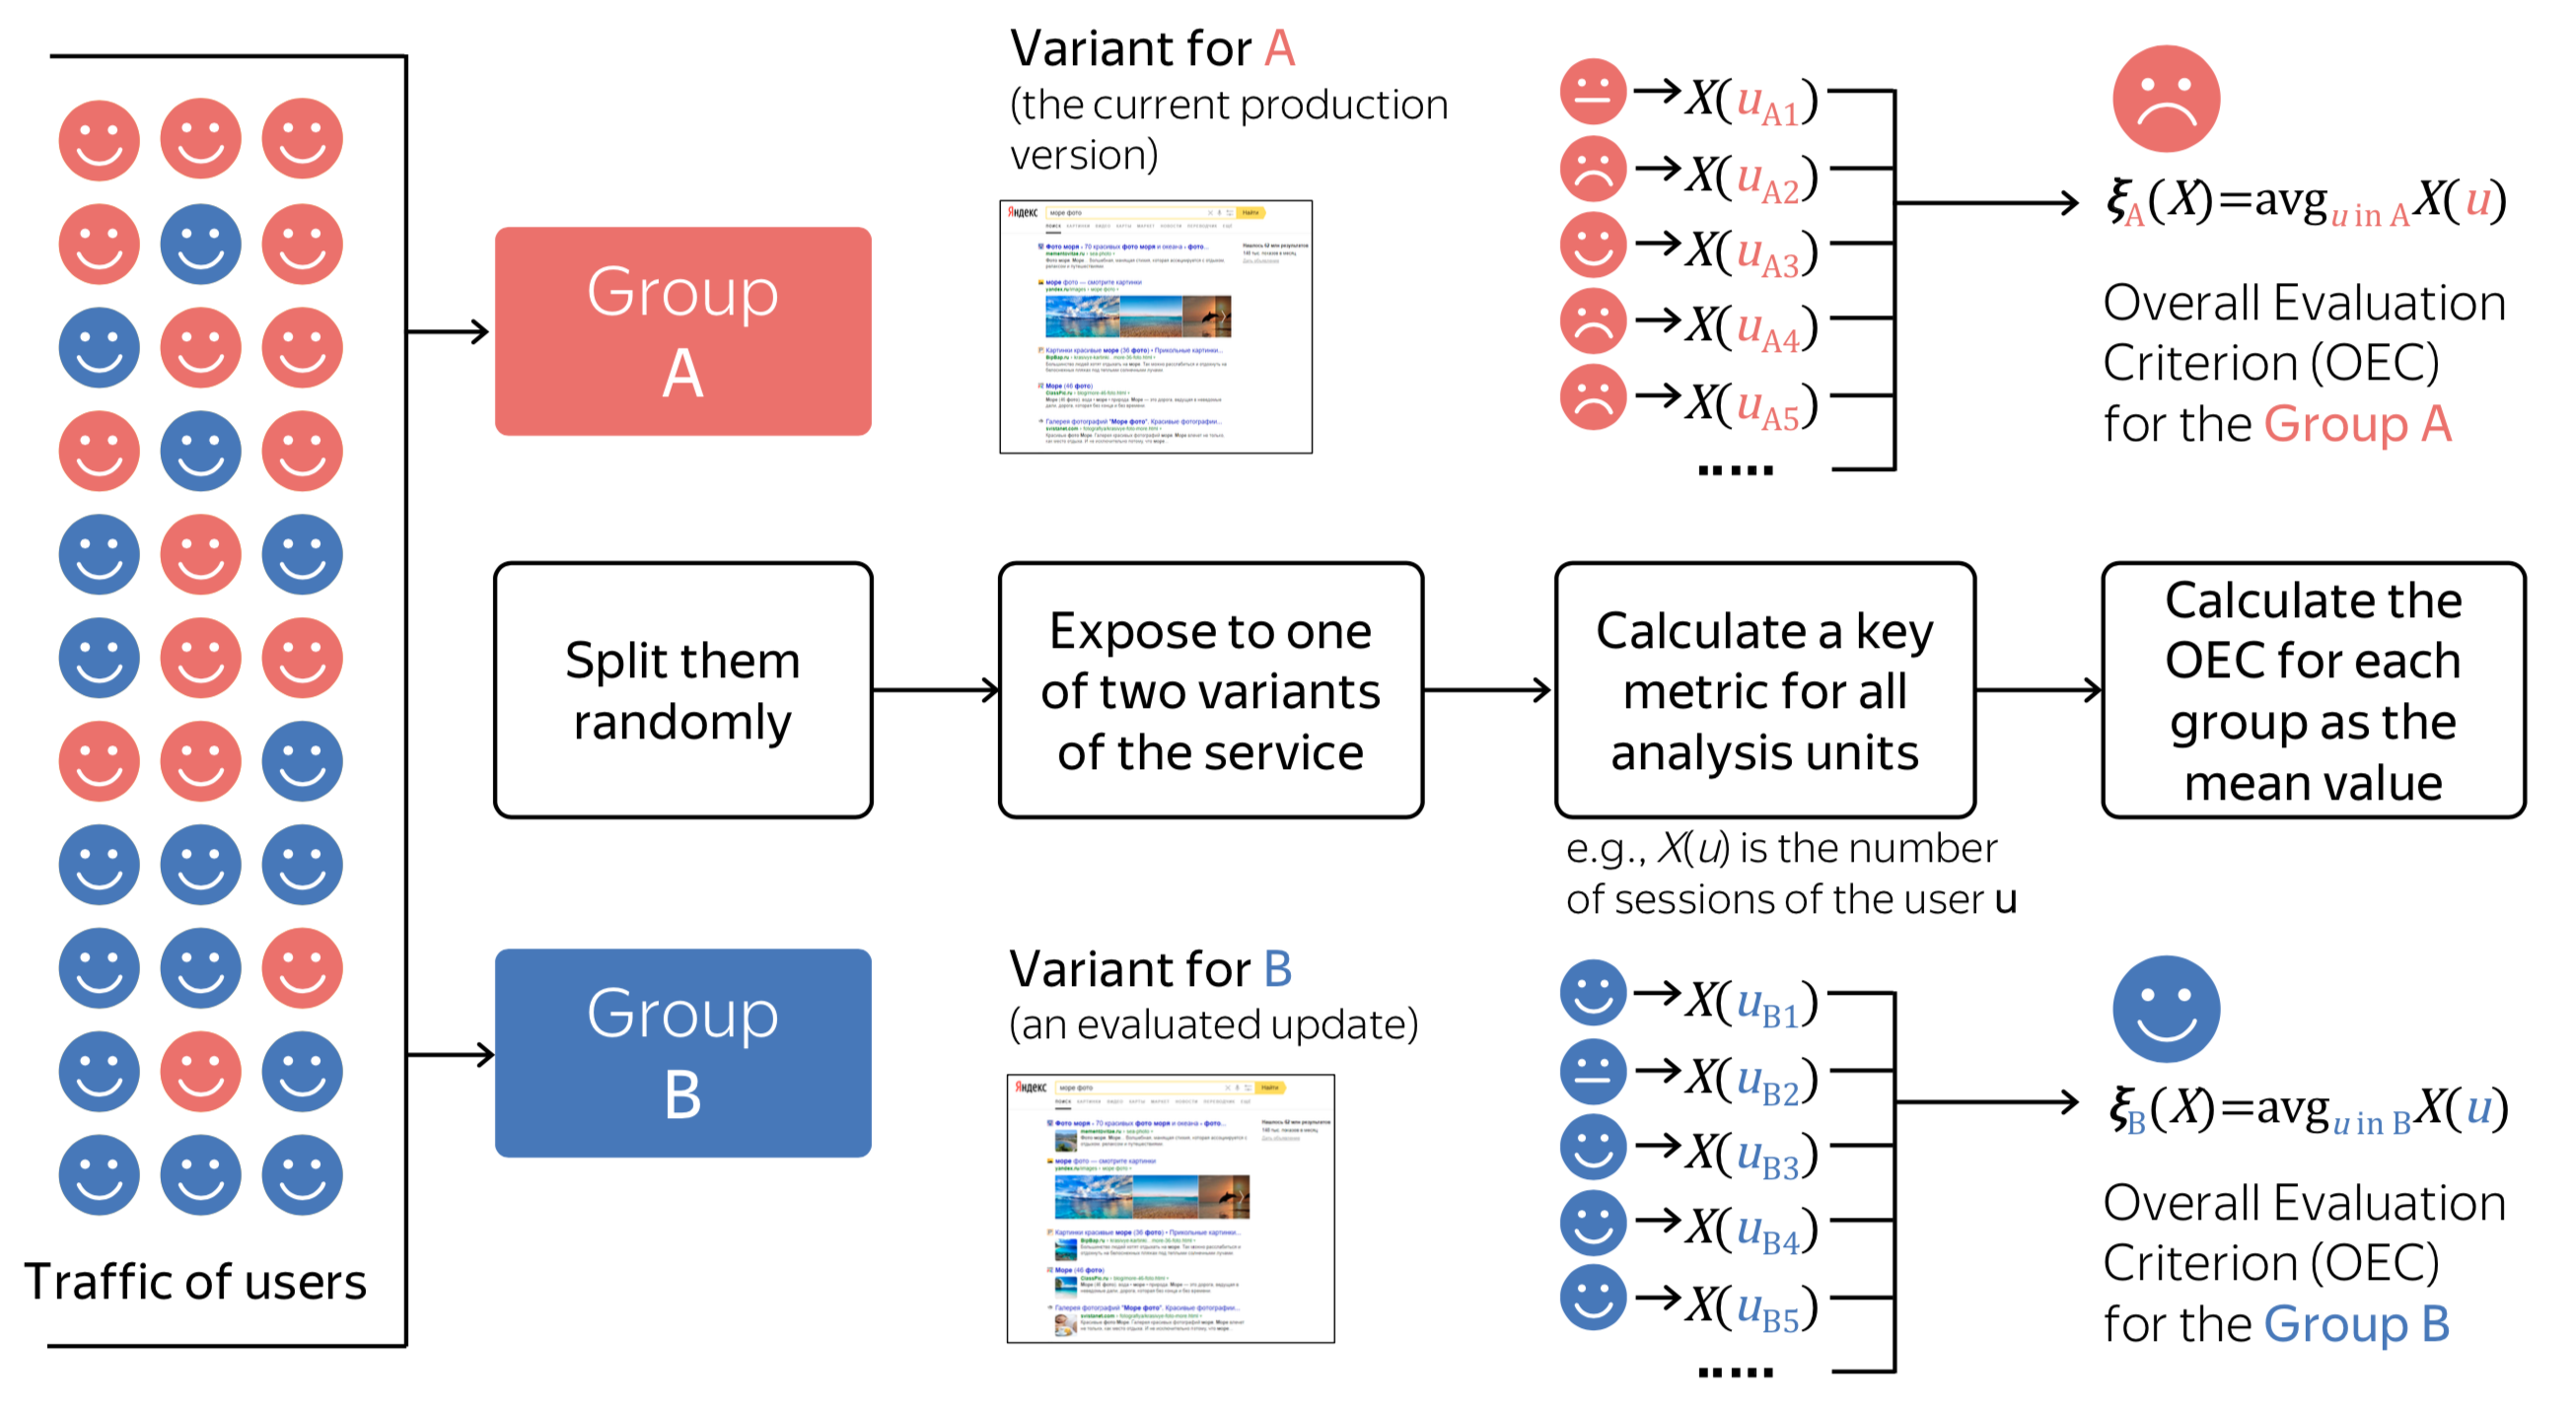
\includegraphics[width=0.5\textwidth]{figures/online_eval_AB_testing.png}
		\caption{Visualization of A/B Testing}
		\label{img:online_eval_AB_testing}
	\end{figure}
\end{itemize}
\subsection{Interleaving}
\begin{itemize}
	\item A/B testing introduces a high variance by letting different users evaluate different systems $\implies$ Show interleaved results from both algorithms A and B without telling the user which document is from which model
	\item The evaluation is based on the clicks of a user where the algorithm gets the credit that provided the clicked document
\end{itemize}
\subsubsection{Balanced interleaving}
\begin{itemize}
	\item In balanced interleaving, we select randomly which algorithm starts (A or B). If A would start, we take the first document of A and place it in our interleaved ranking list. Then we pick the first document of B and continue with A again
	\item If a document is already in the interleaved ranking, we skip this document and continue with picking the next document from the \textit{other} ranking model 
	\begin{figure}[ht]
		\centering
		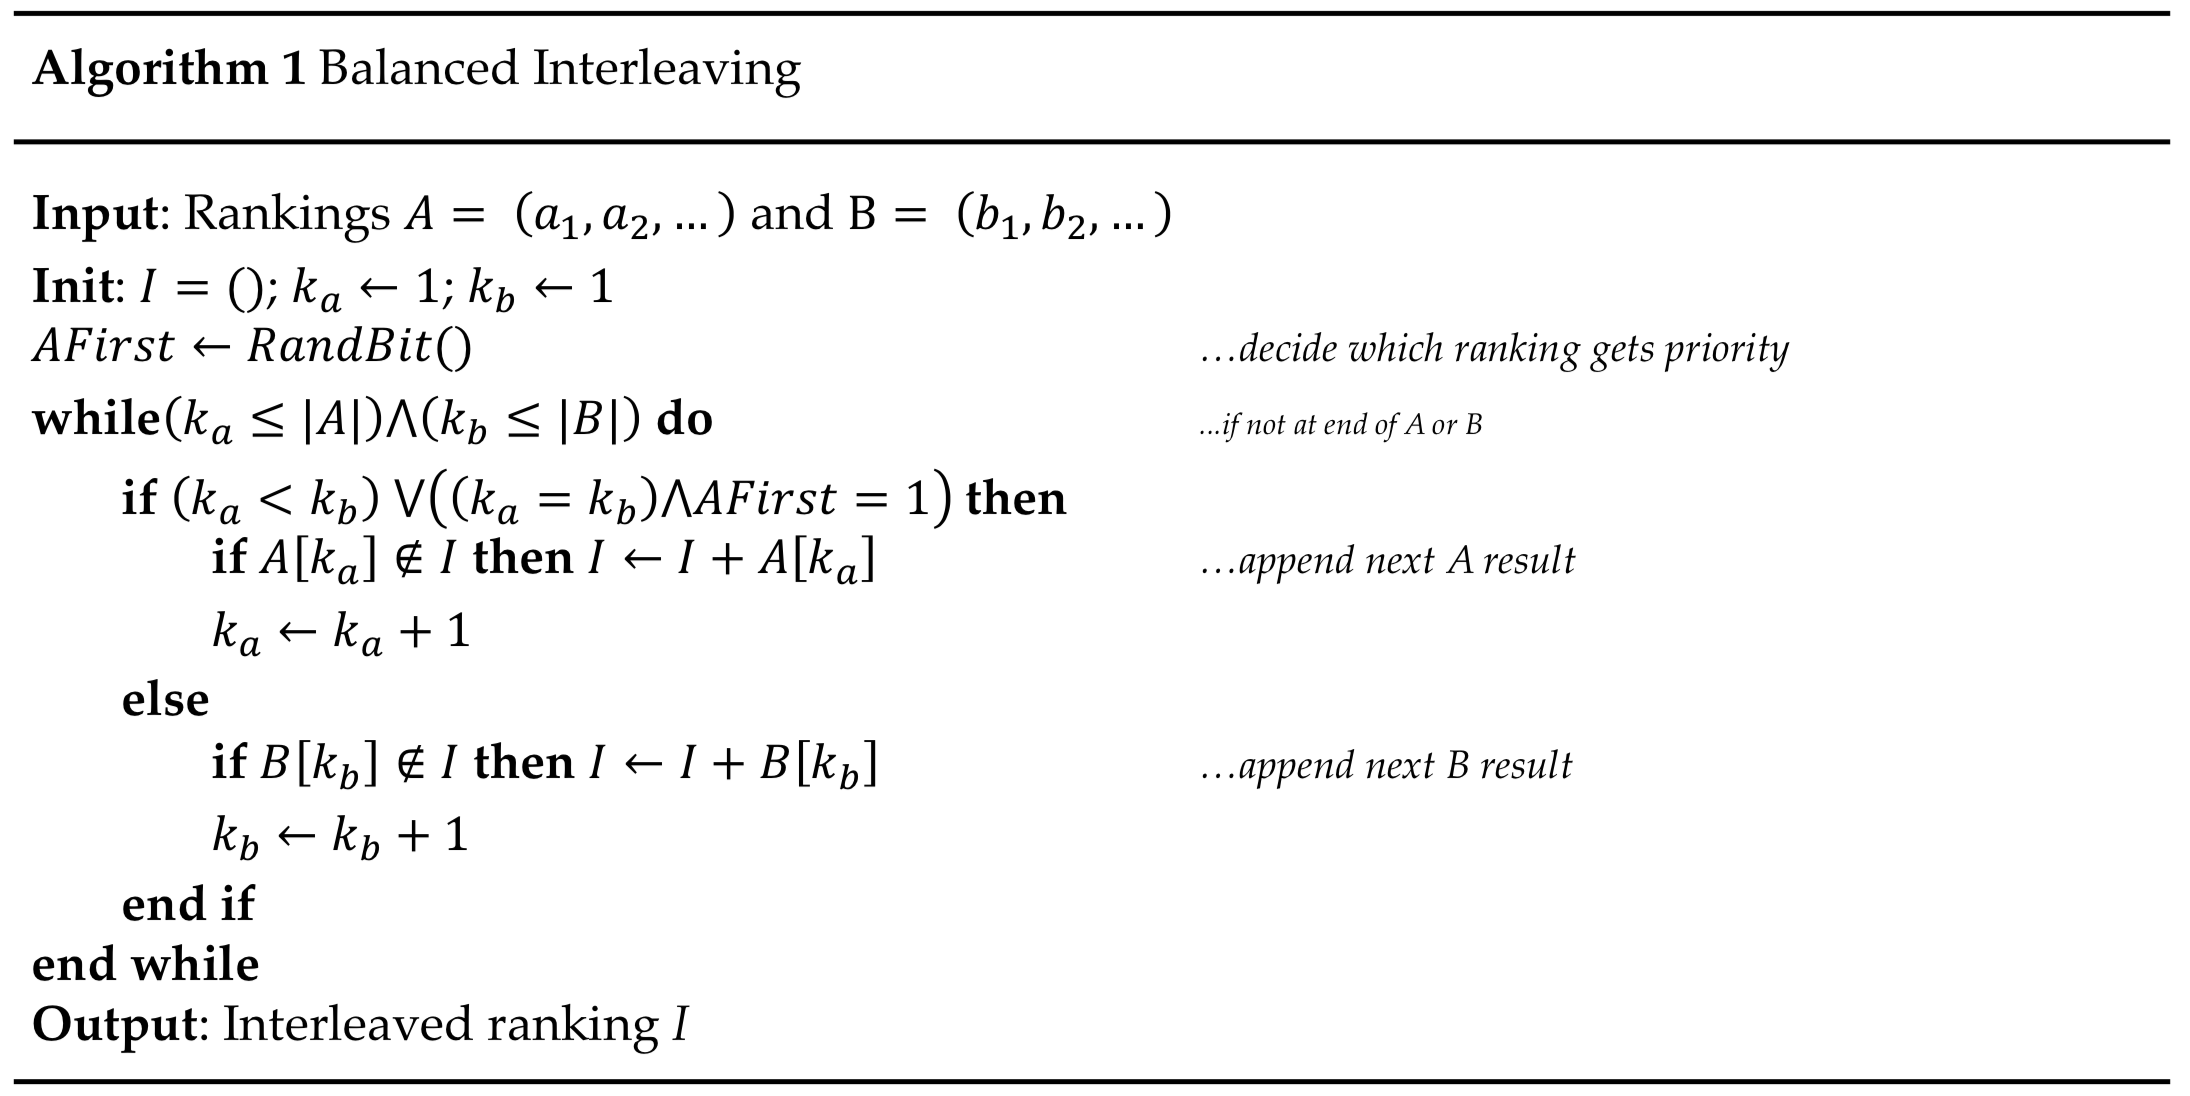
\includegraphics[width=0.5\textwidth]{figures/online_eval_balanced_interleaving.png}
		\caption{Formal algorithm describing balanced interleaving}
		\label{img:online_eval_balanced_interleaving}
	\end{figure}
	\item Problem: balanced interleaving brakes under corner cases. Assume following ranking:
	$$A: \left\{d_1, d_2, d_3, d_4\right\}, B: \left\{d_2, d_3, d_4, d_1\right\}$$
	No matter whether we start at model A or B, the interleaved list contains three documents assigned to B and only one to A. Thus, random clicking would lead to B winning $\implies$ bias. Resolved by team-draft interleaving
\end{itemize}
\subsubsection{Team-draft interleaving}
\begin{itemize}
	\item In team-draft interleaving we guarantee that both algorithms contribute equally to the interleaved ranking
	\item At each stage, we flip a coin to determine whether to pick the next document from A or B first. Afterwards, the document of the other system is picked
	\item If a document is already in the interleaved ranking, we look for the next document from the \textit{same} ranking model until we find a new document.
	\begin{figure}[ht]
		\centering
		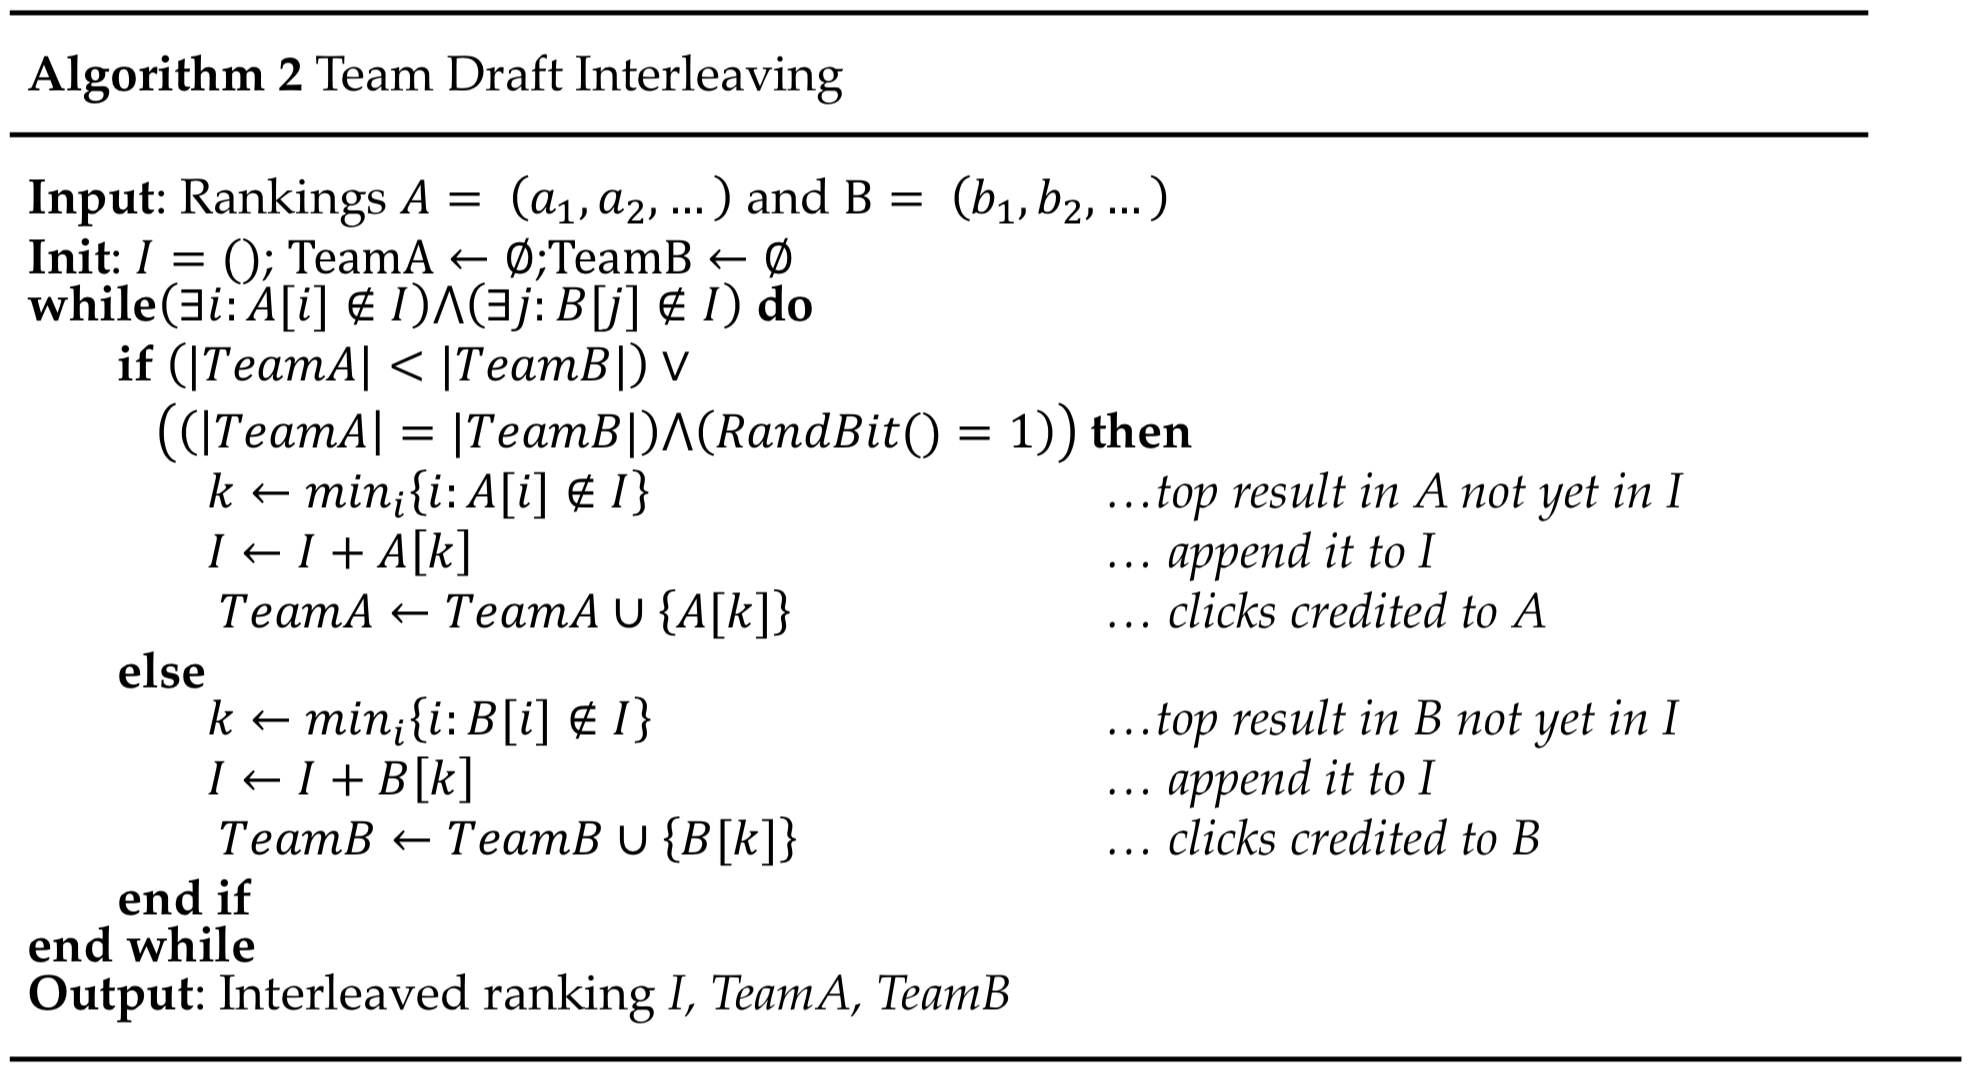
\includegraphics[width=0.5\textwidth]{figures/online_eval_team_draft_interleaving.png}
		\caption{Formal algorithm describing Team-draft interleaving}
		\label{img:online_eval_team_draft_interleaving}
	\end{figure}
	\item There are also corner cases that can cause troubles in team-draft interleaving. However, in practice this rarely happens/has a significant effect. 
\end{itemize}
\subsubsection{Probabilistic interleaving}
\begin{itemize}
	\item To avoid biases completely, we can apply probabilistic models
	\item Convert the ranking of each model to a probability distribution by applying softmax ($\tau = 3$):
	$$p_i(d) = \frac{\frac{1}{r_i(d)^{\tau}}}{\sum_{d' \in D} \frac{1}{r_i(d')^{\tau}}}$$
	\item For every position in the interleaved ranking, flip a coin to determine whether to pick a document from A or B. Next, we sample from the corresponding softmax distribution a document without replacement, and add it to the interleaved list. The picked document is removed from the probability distributions of A and B. 
	\item We can perform evaluation by counting the clicks for documents sampled from A and B. We expect the same number of clicks for documents at the same position of both algorithms due to the same probability in the softmax. % both A and B based on the softmax, and compare which one has the higher probability sum of all clicked documents. Thus, for documents at the same rank, we expect a tie.
	\item Note that compared to a hard assignment of 0 or 1 in balanced and team draft interleaving, the distribution of credit accumulated for clicks is smoothed based on the relative rank of the document in the original result lists (a click on any document leads to a non-zero credit for both rankings)
	\item The algorithm is summarized in Figure~\ref{img:online_eval_probabilistic_interleaving}
	\begin{figure}[ht]
		\centering
		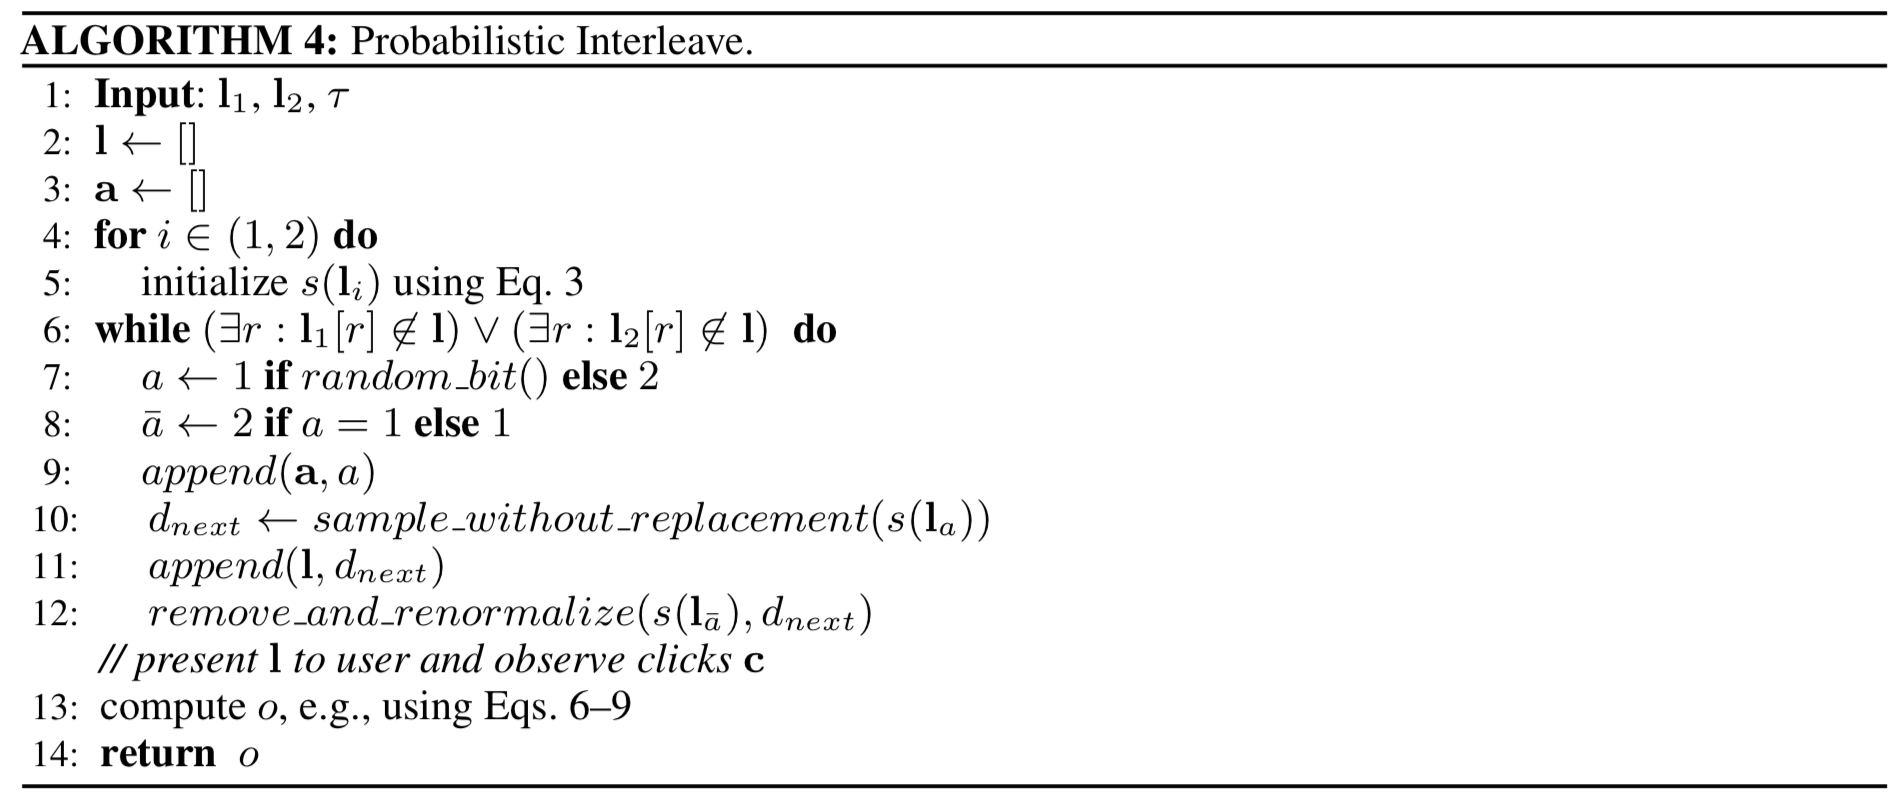
\includegraphics[width=0.5\textwidth]{figures/online_eval_probabilistic_interleaving.png}
		\caption{Formal algorithm describing probabilistic interleaving}
		\label{img:online_eval_probabilistic_interleaving}
	\end{figure}
	\item Another, more efficient evaluation method is by marginalizing over all possible assignments $a$. Therefore, we calculate the probability of the interleaved list $l$ given $a$ (and the query $q$) by successively multiplying the softmax probabilities at that point. For example, the first assignment $a=\left\{1,1,1,1\right\}$ leads to the following calculation:
	$$p(l_i|a=\left\{1,1,1,1\right\},q) = 0.85 \cdot \frac{0.1}{0.15} \cdot \frac{0.03}{0.05} \cdot \frac{0.02}{0.02} = 0.34$$
	\item Normalizing all $p(l_i|a,q)$ by its sum lead to $p(a|l_i,q)$ $\implies$ $p(a|l_i,q) = \frac{p(l_i|a,q)}{\sum_{a \in A} p(l_i|a,q)}$
	\item For every assignment, we add the value $o=-1$ times the probability $p(a|l_i,q)$ if more clicked documents were assigned to $A$. If $B$ has more clicks, we use $o=1$ as factor, and ignore it for a tie (or multiply by $o=0$). Thus, our expected number of wins $B$ has more than $A$ is given by:
	$$E[O] = \sum_{a \in A} o_a \cdot p(a|l_i,q) \text{\hspace{2mm}where\hspace{2mm}} o_a = \begin{cases}
	 -1 & \text{if } c_A > c_B\\
	 0 & \text{if } c_A = c_B\\
	 1 & \text{if } c_A < c_B
	\end{cases}$$
	\item Figure~\ref{img:online_eval_probabilistic_interleaving_2} visualizes an example for probabilistic interleaving
	\begin{figure}[ht]
		\centering
		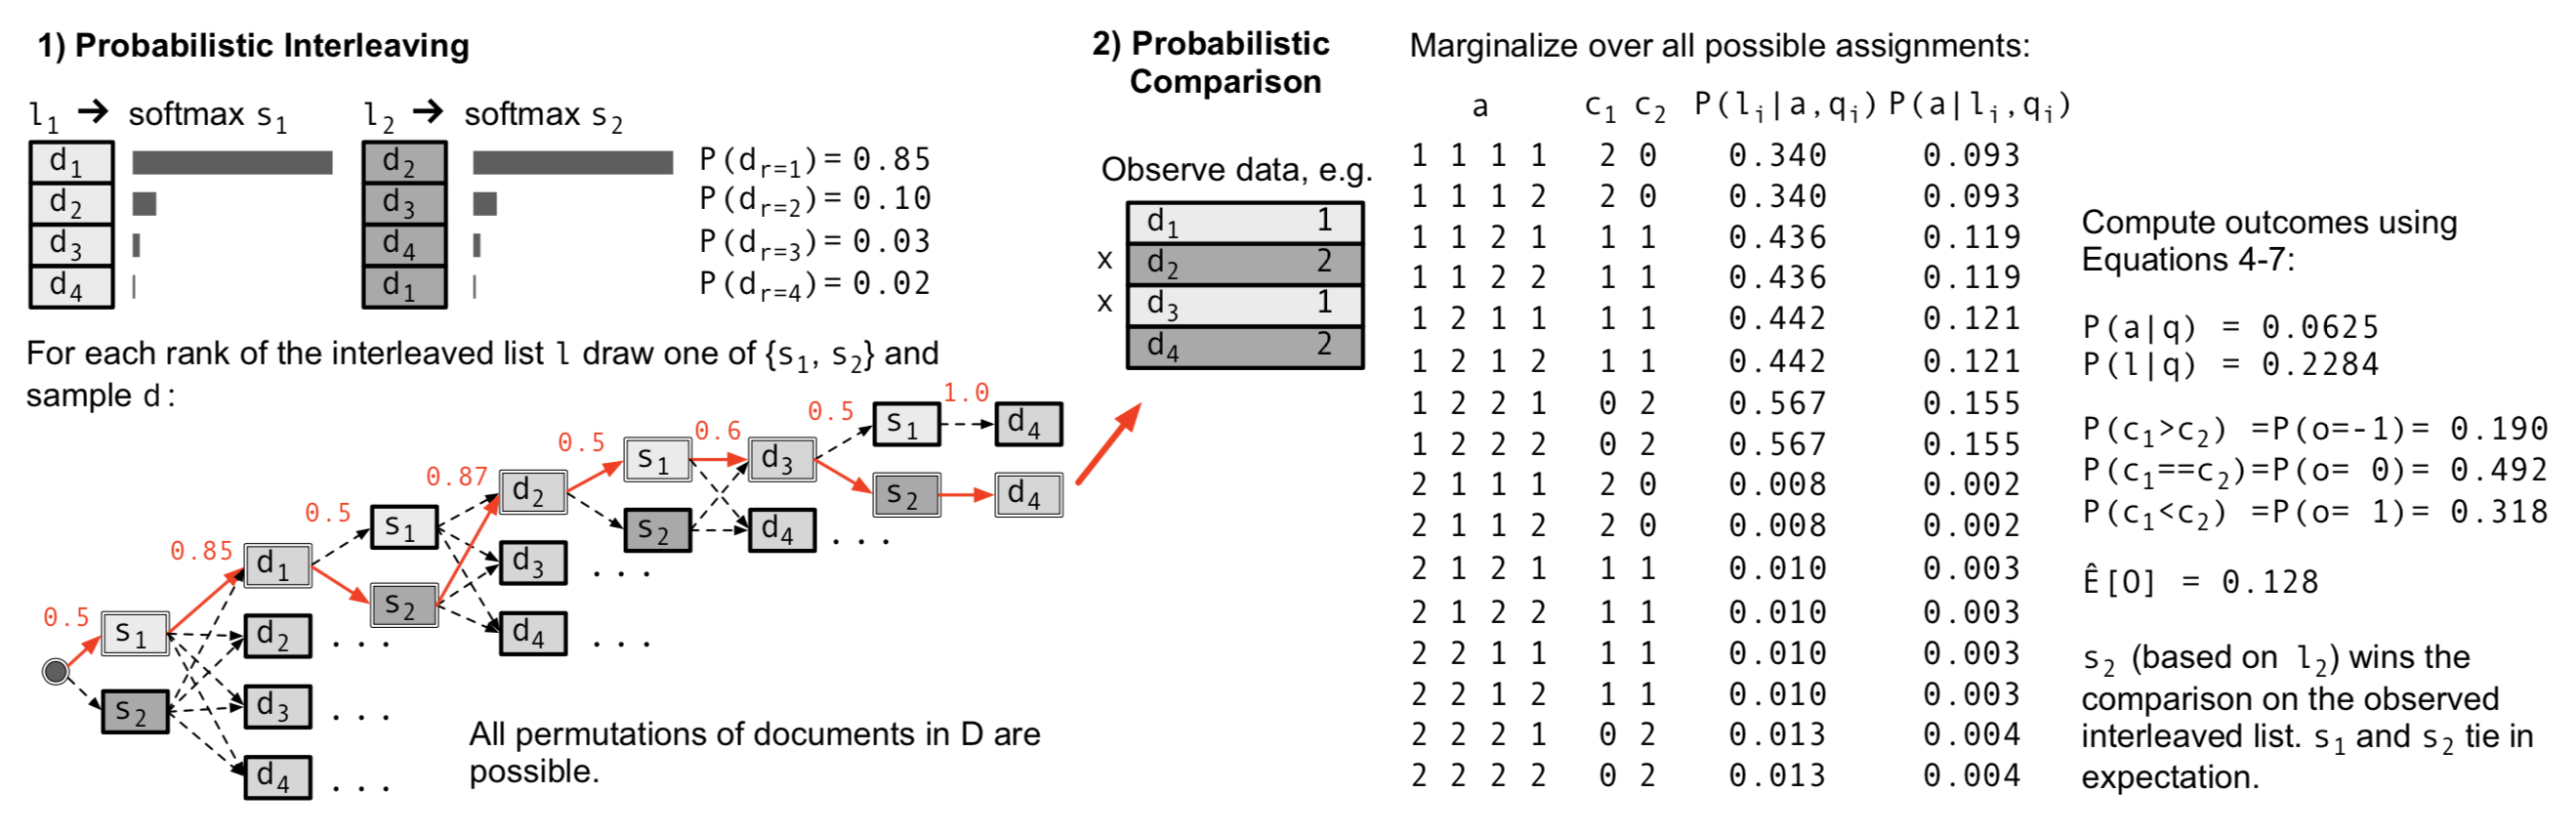
\includegraphics[width=\textwidth]{figures/online_eval_probabilistic_interleaving_2.png}
		\caption{Visualization of probabilistic interleaving}
		\label{img:online_eval_probabilistic_interleaving_2}
	\end{figure}
\end{itemize}